\documentclass{subfiles}
\begin{document}
La convoluzione è un operatore lineare, e in quanto tale soddisfa l'\emph{Equazione \ref{eq:1}}.
Essa può essere utilizzata in vari modi, ma tutti sono accomunati da un elemento comune il \emph{kernel}.
In maniera sintetica, si pensi al kernel come una finestrella che isola parte dell'immagine.

\subsubsection{Filtro di convoluzione blur}
Un filtro di convoluzione blur, o filtro di media, come suggerisce il nome, sfoca l'immagine.
Partendo da un immagine \(I\), avendo un kernel \(K\), si procede a creare una nuova immagine \(I'\), secondo quanto segue.
\\ \\
Si sovrappone il kernel \(K\) all'immagine \(I\), partendo dal pixel più in alto a sinistra;
si effettua un prodotto prodotto punto-punto tra il kernel e l'immagine, si sommano tali valori e lo si divide per il numero di elementi del kernel;
in una nuova immagine \(I'\), nelle coordinate dell'elemento centrale del kernel, si aggiunge un pixel il cui colore è dato dalla media precedentemente calcolata.
Si procede analogamente per tutti i pixel dell'immagine, spostandosi di un pixel verso destra di volta in volta e ripartendo dall'estrema sinistra della riga successiva,
ogni volta che una è completata.\\

\begin{wrapfigure}[12]{r}{0.45\textwidth}
    \centering
    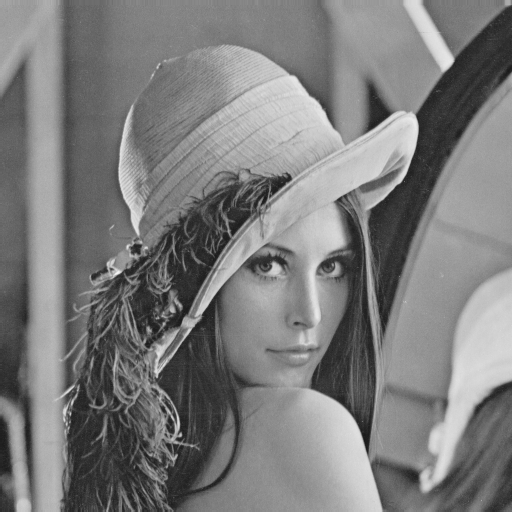
\includegraphics[scale = 0.25]{../Images/LenaGS.png}
    \caption{LenaGS}
    \label{fig:4.1}
\end{wrapfigure}
\noindent Si consideri \emph{Figura \ref{fig:4.1}}, e si supponga di dovervi applicare una sfocatura.
Si consideri dunque un primo tentativo di sfocatura, utilizzando il seguente kernel
\[K = \begin{pmatrix}
        0 & 4 & 0 \\
        4 & 8 & 4 \\
        0 & 4 & 0 \\
    \end{pmatrix}\]

\begin{wrapfigure}{l}{0.4\textwidth}
    \centering
    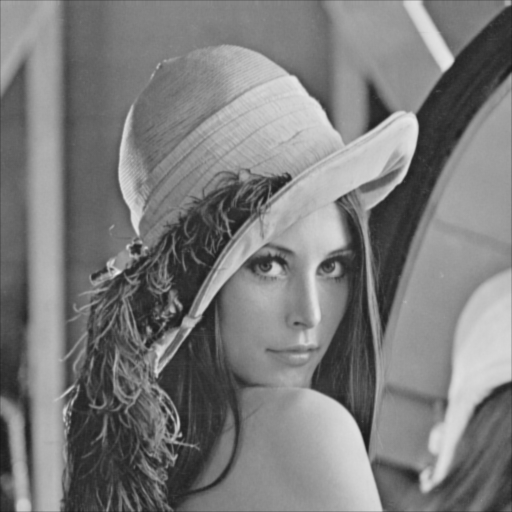
\includegraphics[scale = 0.25]{../Images/MeanConvolutionLena.png}
    \caption{Convoluzione di \emph{Figura \ref{fig:4.1}}, tramite kernel K.}
    \label{fig:4.2}
\end{wrapfigure}
\begin{Remark*}
    Con il filtro di cui sopra la sfumatura è appena percettibile, come sarà più evidente dalle successive versioni,
    al cambiare del kernel, sia nelle sue dimensioni, sia nei pesi dello stesso, si ottiene una sfocatura diversa.
\end{Remark*}

\noindent Eseguendo l'opportuno codice MATLAB, di seguito riportato, ciò che si ottiene è quanto in \emph{Figura \ref{fig:4.2}}.
\begin{center}
    \begin{lstlisting}[language = MATLAB]
        % si aggiunge l'immagine trascinandola in MATLAB
        ker = [0 4 0; 4 8 4; 0 4 0]/24;
        convLena = conv2(single(Lena), ker, `same');
        figure; imshow(uint8(convLena), [0, 255]);
    \end{lstlisting}
\end{center}

\noindent Analizzando il codice: \lstinline[language = MATLAB]{conv2(single(Lena), ker, `same')} effettua l'effettiva convoluzione tra l'immagine e il kernel,
dove il parametro `same', sta ad indicare che convLena dovrà avere le stesse dimensioni dell'immagine originale;
mentre \lstinline[language = MATLAB]{figure; imshow(uint8(convLena), [0, 255])} permette di visualizzare il risultato.

\begin{Note*}
    il cast a single, corrispettivo del float in C, è necessario per via implementazione della funzione \lstinline[language = MATLAB]{conv2};
    quello a uint8, corrispettivo dell'int in C, non è strettamente necessario.
\end{Note*}
\clearpage

%TODO: Fixa sto aborto
\paragraph{Problema ai bordi}
Legato a questo filtro vi è un problema, il cosiddetto \emph{problema ai bordi}.
Si consideri ora un'alto kernel, ad esempio un kernel 11 x 11 in cui ogni elemento è posto ad 1.\\
Eseguendo il codice MATLAB, a seguire, ciò che ne risulta è l'immagine in \emph{Figura \ref{fig:4.3}}.
\begin{wrapfigure}[12]{r}{0.4\textwidth}
    \centering
    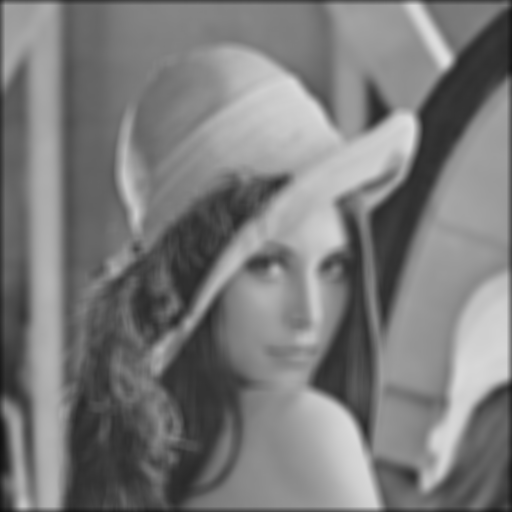
\includegraphics[scale = 0.275]{../Images/MeanConvolutionLena_11x11.png}
    \caption{Convoluzione di \emph{Figura \ref{fig:4.1}}, tramite kernel 11x11 unitario.}
    \label{fig:4.3}
\end{wrapfigure}

\begin{center}
    \begin{lstlisting}[language = MATLAB]
        % si aggiunge l'immagine trascinandola in MATLAB
        ker = ones(11)/121;
        convLena = conv2(single(Lena), ker, `same');
        figure; imshow(uint8(convLena), [0, 255]);
    \end{lstlisting}
\end{center}

\noindent Passando all'analisi del codice: l'istruzione \lstinline[language = MATLAB]{ones(11)} permette di creare una matrice, quindi un kernel, 11 x 11,
i cui elementi sono tutti 1.
\\  \\
Sebbene da \emph{Figura \ref{fig:4.3}} si nota appena, quel che capita è che ai bordi non è possibile applicare convoluzione,
proprio perché ad essere considerato è il pixel le cui coordinate combaciano con l'elemento centrale del kernel.
Inoltre, il problema peggiora tanto più grande è il kernel. Sia sin da subito chiaro che tale problema non ammette una soluzione concreta,
esistono unicamente delle tecniche che permettono di ``alleggerire'' il problema.

\begin{Note*}
    si ponga l'attenzione sugli esempi di codice MATLAB, in entrambi i casi il kernel è moltiplicato per l'inverso della somma dei pesi dello stesso,
    effettuando pertanto una media pesata.
\end{Note*}



%TODO: Aggiungere ``soluzioni'' al problema ai bordi.
\end{document}